\documentclass[tikz,border=8pt]{standalone}
\usepackage{amsmath}
\usetikzlibrary{arrows.meta,calc}

\begin{document}
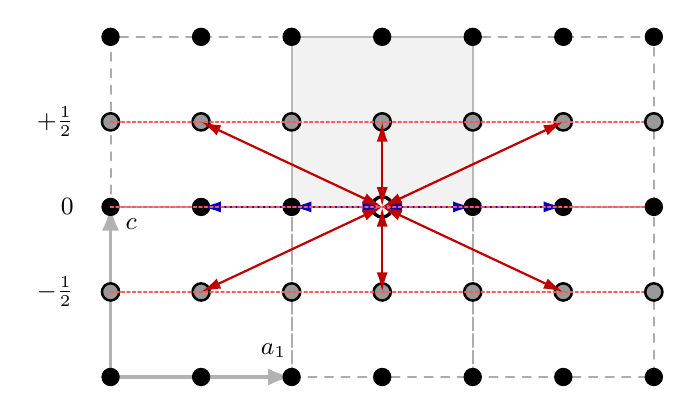
\begin{tikzpicture}[
    x=1.15cm, y=0.9cm,
    line cap=round, line join=round,
    cell/.style={draw=gray!65, dash pattern=on 3pt off 3pt, line width=0.7pt},
    cellhl/.style={draw=gray!55, line width=0.8pt, fill=gray!10},
    plane/.style={draw=red!65, dash pattern=on 1pt off 1pt, line width=0.7pt},
    siteA/.style={circle, fill=black, draw=black, inner sep=2.2pt},
    siteB/.style={circle, fill=black!40, draw=black, line width=0.9pt, inner sep=2.2pt},
    vac/.style={circle, fill=white, draw=black, line width=1.2pt, inner sep=2.6pt},
    vec/.style={very thick, draw=gray!60, -{Latex[length=3mm,width=2.2mm]}},
    basal/.style={thick, draw=blue!75!black, {Latex[length=2.5mm,width=1.4mm]}-{Latex[length=2.5mm,width=1.4mm]}},
    inter/.style={thick, draw=red!75!black, {Latex[length=2.5mm,width=1.4mm]}-{Latex[length=2.5mm,width=1.4mm]}},
    lbl/.style={font=\small}
]

\def\a{2}
\def\c{2.4}
\coordinate (a1) at (\a,0);
\coordinate (cvec) at (0,\c);

% Draw the cell grid extended by one cell in x, without the upper row of cells; keep the y=1 row of atoms.
\foreach \i in {-1,0,1} {
  \foreach \j in {-1,0} {
    \coordinate (P\i\j) at ({\i*\a}, {\j*\c});
    \draw[cell] (P\i\j) -- ($(P\i\j)+(a1)$) -- ($(P\i\j)+(a1)+(cvec)$) -- ($(P\i\j)+(cvec)$) -- cycle;
  }
}

% central primitive cell
\draw[cellhl] (0,0) -- (a1) -- ($(a1)+(cvec)$) -- (cvec) -- cycle;

% draw lattice vectors in the lower-left neighboring cell, not in the central cell
\coordinate (v0) at (-\a,-\c);
\coordinate (v1) at (0,-\c);
\coordinate (vc) at (-\a,0);
\draw[vec] (v0) -- (v1);
\draw[vec] (v0) -- (vc);
\node[lbl, anchor=north] at (0.1*\a - 0.2*\a, -0.75*\c) {$a_1$};
\node[lbl, anchor=west] at (-0.97*\a, -0.1*\c) {$c$};

% phase labels for basal planes, shifted slightly left so they are not hidden by the spheres.
% Only the in-loop values are labelled.
\foreach \phase/\y in {{-\tfrac12}/{-0.5*\c}, {0}/{0}, {+\tfrac12}/{0.5*\c}} {
    \node[lbl, anchor=east] at ({-1.15*\a}, {\y}) {$\phase$};
}

% Keep the y=1 row of A atoms, remove the two upper rows y=1.5 and y=2.0,
% and add the extra right-hand column at x=2.0 using the same y-levels as the highlighted cell.
\foreach \x in {-1,-0.5,0,0.5,1,1.5} {
    \foreach \y in {-1,0,1} {
        \node[siteA] at ({\x*\a},{\y*\c}) {};
    }
}
\foreach \x in {-1,-0.5,0,0.5,1,1.5} {
    \foreach \y in {-0.5,0.5} {
        \node[siteB] at ({\x*\a},{\y*\c}) {};
    }
}
% The extra right-hand column is green and should be the only material at x=2.0.
% Vacancy; in this projection it lies at the middle of the basal line.
\coordinate (A) at ({0.5*\a}, {0});
\node[vac] at (A) {};

% Blue arrows: same-basal-plane NN in the projected row y=0. Only four are visible
% because the remaining two are overlapped in this 2D projection.
\foreach \x in {-0.5,0,1,1.5} {
    \draw[basal] (A) -- ({\x*\a}, {0});
}

% Red dashed guide lines through the relevant atomic rows, cut on the left of x=-1 and on the right of x=2.
\foreach \y in {-0.5,0,0.5} {
    \draw[plane] ({-\a}, {\y*\c}) -- ({2*\a}, {\y*\c});
}

% Restore the red arrows as before: three grey neighbors above and three below.
\foreach \x in {-0.5,0.5,1.5} {
    \draw[inter] (A) -- ({\x*\a}, {0.5*\c});
    \draw[inter] (A) -- ({\x*\a}, {-0.5*\c});
}

% Restore the normal atom colors/styles: the extra right-hand column uses the same
% row-by-row site types as the rest of the projection.
\foreach \y/\type in {-1/siteA,-0.5/siteB,0/siteA,0.5/siteB,1/siteA} {
    \node[\type] at ({2*\a},{\y*\c}) {};
}

\end{tikzpicture}
\end{document}
